\documentclass[12pt]{article}
\date{October~2,~2010}
%\documentstyle[12pt,epsfig,rotate]{article}
\input epsf
\pagestyle{headings}
\usepackage{fullpage}
\usepackage{multirow}
\usepackage{caption}
\usepackage{graphicx}
\usepackage{subfig} % Neccessary for subfigures, needs to be installed
\usepackage{hyphenat}
\usepackage{color,fancyvrb}
\usepackage{setspace}
\usepackage{amsmath}
%\usepackage[pdftex]{graphics}
\def\beqn{\begin{eqnarray}}
\def\eeqn{\end{eqnarray}}

%\pdfpagewidth 7.0in
%\pdfpageheight 9.2in
\setlength\topmargin{0.6in}
%\setlength\headheight{0in}
%\setlength\headsep{0in}
\setlength\textheight{8.5in}
\setlength\textwidth{6.0in}
%\setlength\oddsidemargin{-.5in}
%\setlength\evensidemargin{-.5in}
%\setlength\parindent{0in}
%\setlength\parskip{0in} 
\textwidth  5.5in
\textheight 9.5in
\topmargin 0.8 in
%\oddsidemargin 0.4in
%\evensidemargin 0.4in
%\pagestyle{headings}
%\pagenumbering{arabic}
\newcommand{\Thgg}{$\theta_{\gamma^*\gamma}~$}
\newcommand{\Phgg}{$\phi_{\gamma^*\gamma}~$}
\newcommand{\Epg}{$ep~\rightarrow~ep\gamma~$}
\newcommand{\Eppiz}{$ep~\rightarrow~ep\pi^o~$}
\newcommand{\Enpip}{$ep~\rightarrow~en\pi^+~$}
\newcommand{\EppiD}{$ep~\rightarrow~e\pi \Delta~$}
\newcommand{\Epeta}{$ep~\rightarrow~ep\eta~$}
\newcommand{\Epr}{$ep~\rightarrow~ep\rho~$}
\newcommand{\EpX}{$ep~\rightarrow~epX~$}
\newcommand{\EpKY}{$ep~\rightarrow~eKY~$}
\newcommand{\vEpg}{$\vec ep~\rightarrow~ep\gamma~$}
\def\gevc2{(GeV/c)$^2$}
%\vspace{-1.4cm}
\begin{document}
\pagestyle{plain}
\pagenumbering{arabic}
%\indent
%\input{central_introduction.tex}
%\input{central_solenoid.tex}
%\input{central_tracker.tex}
%\input{central_tof.tex}%
%\input{central_ec.tex}%
%\begin{thebibliography}{99}
%% \bibitem{CLAS12G}

\bibitem{BONUS} JLab E03-12, The Structure of the Free Neutron Via Spectator 
Tagging. H. Fenker, C. Keppe, S. Kuhn and W. Melnitchouk spokespersons.  

\bibitem{ZHENG}
X. Zheng {\it et al.},
Phys. Rev. Lett. {\bf 92}, 012004 (2004);
Phys. Rev.  {\bf C70} 065207 (2004).

\bibitem{VIPULI} K.V. Dharmawardane {\it et al.},
Phys.Lett. {\bf B641} 11 (2006).

\bibitem{BONUS12} JLab  E12-06-113, The Structure of the Free Neutron at 
Large x-Bjorken. S. Bueltmann, M. Christy, H. Fenker, K. Griffioen, 
C. Keppel, S. Kuhn, W. Melnitchouk, V. Tvaskis spokespersons.  

\bibitem{EG12} E12-06-109 The Longitudinal Spin Structure of the Nucleon. 
D. Crabb, A. Deur, K. Dharmawardane, T. Forest, K. Griffioen, M. Holtrop, 
S. Kuhn, Y. Prok

\bibitem{KUHL}
S.~Kuhlmann {\em et al.},
Phys. Lett. B {\bf 476}, 291 (2000).

\bibitem{MT}
W.~Melnitchouk and A.~W.~Thomas,
Phys. Lett. B {\bf 377}, 11 (1996).

\bibitem{Leader:2005ci}
  E.~Leader, A.~V.~Sidorov and D.~B.~Stamenov,
  %``Longitudinal polarized parton densities updated,''
  Phys.\ Rev.\ D {\bf 73}, 034023 (2006)
  [arXiv:hep-ph/0512114].
  %%CITATION = HEP-PH 0512114;%%

\bibitem{Dharmawardane:2006zd}
  K.~V.~Dharmawardane, S.~E.~Kuhn, P.~Bosted and Y.~Prok  [the CLAS
                  Collaboration],
  %``Measurement of the $x$- and $Q^2$-Dependence of the Asymmetry $A_1$ on the
  %Nucleon,''
  to be published in Phys. Lett., arXiv:nucl-ex/0605028.
  %%CITATION = NUCL-EX 0605028;%%


 \bibitem{EG1a}
R. Fatemi {\it et~al.} [CLAS Collaboration],
Phys. Rev. Lett. {\bf 91}, 222002 (2003),
J. Yun  {\it et~al.} [CLAS Collaboration],
Phys. Rev. C {\bf 67}, 055204 (2003).

\bibitem{rev_mom}
J.-P. Chen, A. Deur, Z.-E. Meziani, Mod. Phys. Lett. \textbf{A20}, 2745 (2005);
M. Osipenko {\it et al.}, Phys. Rev. D {\bf 71}, 054007 (2005).


\bibitem{Bj}
J. D. Bjorken, Phys. Rev. \textbf{148}, 1467 (1966).

\bibitem{GDH}
S. D. Drell and
A. C. Hearn, Phys. Rev. Lett. \textbf{16}, 908 (1966);
S. Gerasimov, Sov. J. Nucl. Phys. \textbf{2}, 430 (1966).

\bibitem{JiSR}
X. Ji and J. Osborne, J. Phys. {\bf G27} 127 (2001).

\bibitem{HERMES}
HERMES collaboration: A. Airapetian \emph{et al.}, 
Eur. Phys. J. {\bf C26}, 527 (2003).

\bibitem{E143}
E143 collaboration: K. Abe \emph{et al.},
Phys. Rev. Lett. \textbf{78}, 815 (1997); 
K. Abe \emph{et al.}, 
Phys. Rev. D {\bf58}, 112003 (1998).

\bibitem{E155}
P.L. Anthony {\it et al.,} Phys. Lett. {\bf B493}, 19 (2000).

\bibitem{AO}
V. D. Burkert and B. L. Ioffe,
Phys. Lett. \textbf{B296}, 223 (1992);
J. Exp. Theor. Phys. {\bf 78}, 619 (1994).

\bibitem{BT} N. Bianchi and E. Thomas,
Nucl. Phys. Proc. Suppl. \textbf{82}, 256 (2000).

\bibitem{BjHT} 
A. Deur {\em et al.}, Phys. Rev. Lett. {\bf 93} 212001 (2004)

\bibitem{E97110} J.P. Chen, A. Deur and F. Garibaldi, JLab experiment
E97-110

\bibitem{E03006} M. Battaglieri, A. Deur, R. De Vita and M. Ripani,
JLab experiment E03-006

\bibitem{BG}
E.~D.~Bloom and F.~J.~Gilman,
Phys. Rev. Lett. {\bf 16}, 1140 (1970);
Phys. Rev. D {\bf 4}, 2901 (1971).

\bibitem{NIC}
I.~Niculescu {\em et al.},
Phys. Rev. Lett. {\bf 85}, 1182, 1186 (2000).

\bibitem{d2n} M. Amarian {\em et al.}, 
Phys. Rev. Lett. {\bf 92} 022301 (2004)


\bibitem{BOSTED EG1b}P.E. Bosted {\it et al.},
hep-ph/0607283


\bibitem{E01-012} P. Solvigon, Contribution to the proceedings of the First 
Workshop on Quark-Hadron Duality and the Transition to pQCD. A. Fantoni, 
S. Luiti and O. Rondon ed. World Scientific, 2006.


\bibitem{ERIC}
M.~E.~Christy {\em et al.},
E94-110 Collaboration, in preparation.

\bibitem{osipenko} 
M. Osipenko {\em et al.}, Phys. Rev. {\bf D67} 09201 (2003)

\bibitem{noi} 
S. Simula and M. Osipenko, Nucl. Phys. {\bf B675} 289 (2003)

\bibitem{alpha} S. Bethke, $\alpha_S$ 2002 High-Energy Physics Int'l 
Conference in Quantum Chromodynamics, Montpellier (France) (2002)

\bibitem{GDH04} K. Helbing. Talk given at the GDH04 symposium. 
www.physics.odu.edu/GDH2004/Proceedings/Helbing.pdf

\bibitem{SLACGDH} SLAC experiment E159. P. Bosted and D. Crabb spokespersons.
www.slac.stanford.edu/exp/e159/prop.pdf

 
\bibitem{DGP}
A.~de~R\'ujula, H.~Georgi and H.~D.~Politzer,
Ann. Phys. {\bf 103}, 315 (1975).

\bibitem{DUALMODEL}
N.~Isgur, S.~Jeschonnek, W.~Melnitchouk and J.~W.~Van Orden,
Phys. Rev. D {\bf 65}, 054005 (2001).


%\end{thebibliography}
\title
{\vspace{-.2cm}
\begin{flushright}
\normalsize{Draft of NIM paper ~~~~~~~~}
\end{flushright}
\bigskip 
\bigskip
\bigskip
%\begin{center}
Dynamic Magnetic Shield with shield factor of 
 10000 at 1000 Gauss axial fields  \\
for the  Photo Multiplier Tubes of {\tt CLAS12} Central {\tt TOF} Detector.}
%\end{center}
\author
{
{}\\
\mbox
{V.Baturin, V.Burkert, D.Carman, L.Elouadrhiri, D.Grilli, }\\
{ L.Quattier, E.Pasyuk and B.Wieland.}\\
%{and}\\
%{B. Wieland.}
%{N.Harrison, F.Landry, T.Madlem, R.Newcomb,B.Wieland}
{}  \\
\mbox
{}\\
{}\\
}
\maketitle
\begin{abstract}
The Central Time Of Flight detector ({\tt CTOF}) for 12~GeV upgrade 
is being designed at JLab with the  
linear focused   {\tt PMT}s  requiring a robust magnetic shield from the 
 {\tt CLAS12}   main
5~T Solenoid fringe fields of 1000~G. 
Theoretical consideration of a  ferromagnetic 
cylinder in axial field  
has demonstrated  that its  shielding capacity  
decrease  with  increasing length,
i.e. long cylinder does not work efficiently. 
This observation
has been confirmed with Final Element Analysis using  {\tt POISSON} model software.
 Several shields  composed of  coaxial cylinders has been studied.
All  difficulties caused by  saturation effects  
were overcame with a novel dynamical shield, which utilize demagnetizing  solenoids 
between shielding cylinders.
Basic dynamical shields for ordinary linear focused 2'' {\tt PMT}s was  
designed. Its performances were tested both in models and  experimentally, 
at different external fields and demagnetizing currents. Thus designed  
shield meet the performance requirements.  
\end{abstract}
%\begin{flushleft}
%\end{flushleft}
%\newpage 
%\tableofcontents
%\newpage
%\listoftables
%\newpage
%\listoffigures
%\newpage
\section{Introduction.}
The Central Time Of Flight detector ({\tt CTOF}) is being constructed 
at JLab\cite{upgrade2} with 
the  best timing {\tt PMT}s coupled
to the scintillators via  focusing  light guides made of cast acrylic rods.
Conventional linear focused
{\tt R2083} or 
metal channel {\tt H8500} {\tt PMT}s may be  used due to 
their perfect timing characteristics.
Both {\tt PMT}s  exhibit the  transition time spread of $370~ps$ and  the   
rise time of $0.7~ns$, which is close to the rise time of fast scintillators.
  
Linear focused {\tt R2083} is our reference photo detector. 
The layout of one hundred  {\tt PMT}s, and  focusing light guides, and fifty
scintillators  as well,  is shown in Fig.~{\ref{barrel2}}.
The scintillators are  bent from the downstream side and  form a hermetic  barrel,
$66-cm$ long with an inner radius $25~cm$.
% The  corresponding field map of the  solenoid with 
%indicated  locations of {\tt PMT}s is shown in  Fig.~\ref{fig:mmap1}.
%
The nominal field of the {\tt CLAS12}  Solenoid  is $5~T$, therefore 
a very long, straight or  bent, light guides  are used  for  
delivering light to an area outside of the  Solenoid where 
associated high gradient fields  are $ \le1000~G$.

With the triplet of identical  prototyping counters   
we have achieved  the {\tt TOF} resolution of   
$55-60~ps$  at near zero magnetic field, 
using  a double-sided readout\cite{r1}-\cite{6percent}. 
In order to  provide such resolution in real detector 
a robust magnetic shields are required.

Thus, in this paper  we concentrate on the research part of the 
CTOF project aimed for a  robust magnetic shield for the reference photo multiplier. 
We strive  for the  extermination of  the  1~KG external axial  field to 
the level  $\le0.2 G$, that may be considered as a safe environment  
for the timing performance.   
%
\begin{figure}[htbp]
\centering
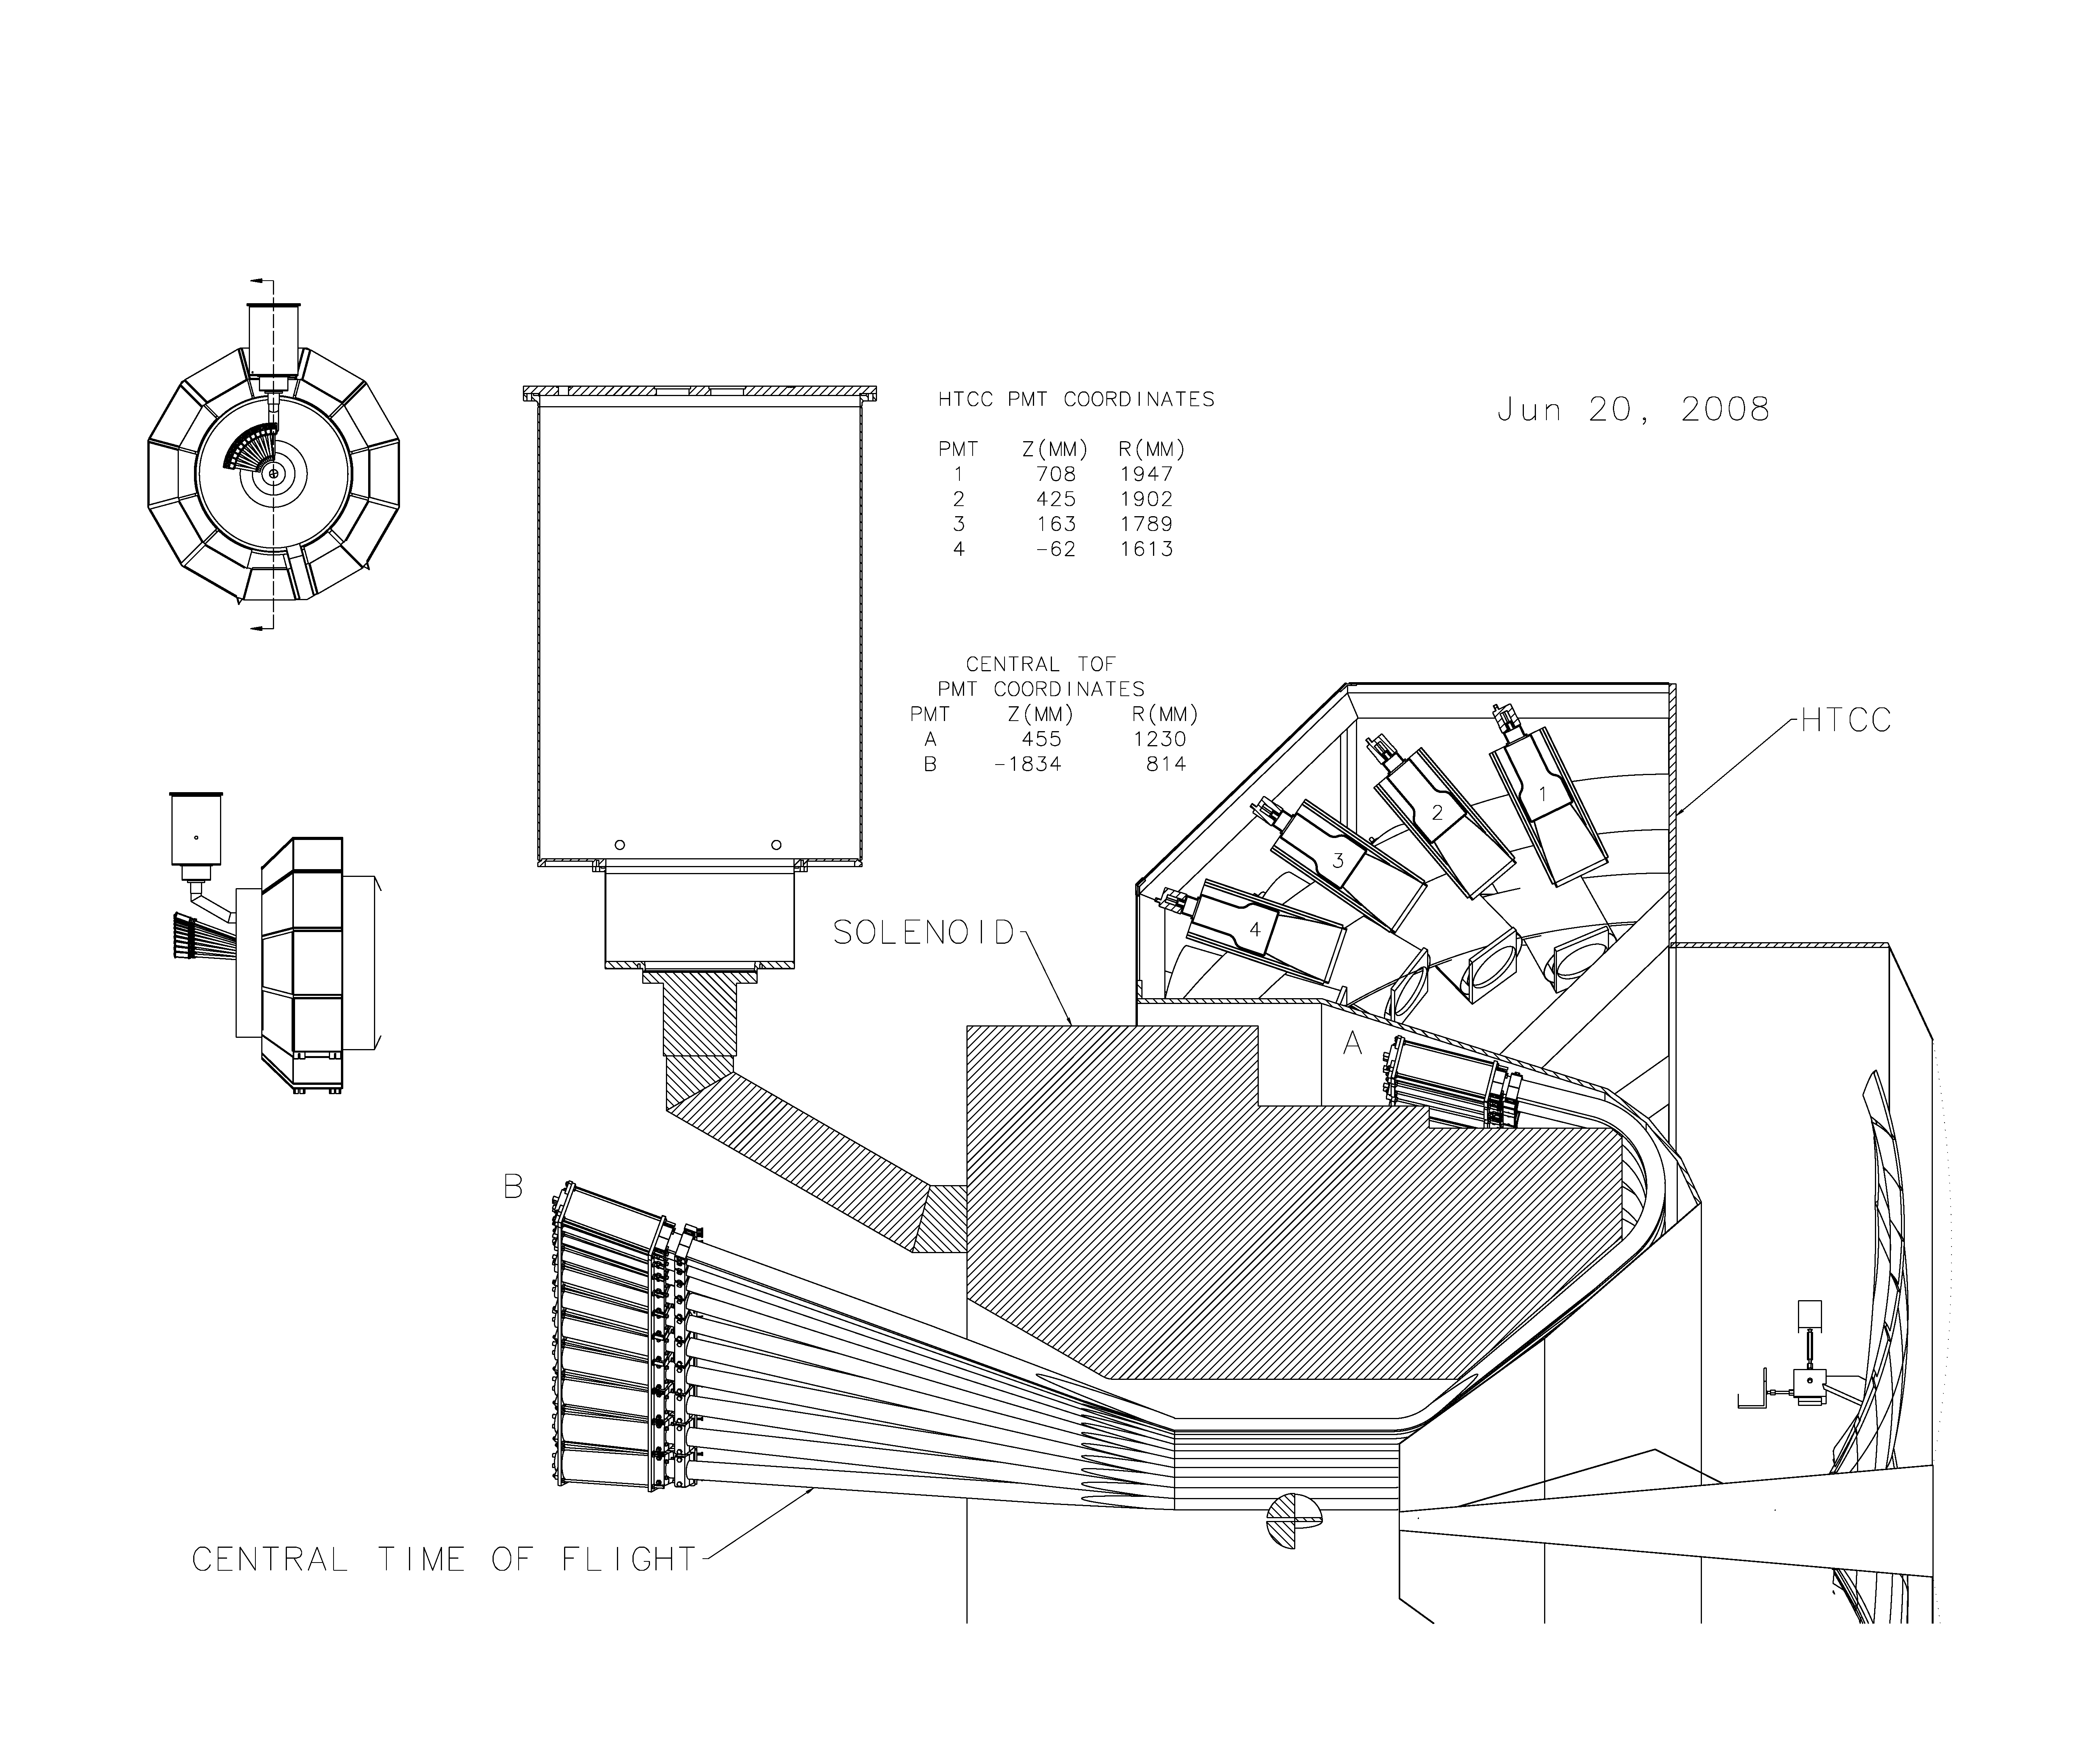
\includegraphics[height=6cm,clip=true,bb= 465 150 2100 1360]{HTCC_CTOF_STUDY_060507_WRAP.eps}
\caption{\small{(a)~The layout of the {\tt CLAS12} {\tt CTOF} detector:
A-downstream {\tt PMT}s, B-upstream {\tt PMT}s, 1,...,4-{\tt PMT}s 
of the High Threshold Cerenkov Counter~({\tt HTCC})}}
\label{barrel2}
\end{figure}
%
With this  goal in mind, we discuss the shield 
constrains and traditional  design principles in Section~\ref{sec:constr} and \ref{sec:principles}.  
In Section~\ref{sec:ednmics},  we describe a simplified  theory 
of a ferromagnetic cylinder in axial field. With this
simple theory  we have  established a 
new effective  principle for the  shield design. 
In the following Section~\ref{sec:fea} we present our 
Final Element Analysis ({\tt FEA}) and  simulations
of various shielding using the  {\tt POISSON} program.
Doing so, we have  verified our design principles and  
designed the desired magnetic shield for our reference {\tt PMT}  in Section~\ref{sec:novelle} 
for both {\tt R2083} and {\tt H8500} {\tt PMT}s.

In Section~\ref{sec:tests} we report on the prototyping shield tests, in particular on 
the shield effectiveness measurements at the axial field  1000~G.
The prospect of using such magnetic shield in the {\tt CTOF} detector 
of {\tt CLAS12} will be discussed in Section~\ref{sec:concl}.   

\section{Design constrains and shield dimensions.}
\label{sec:constr}

\paragraph{Shield diameter.}
Under the current design of the {\tt CTOF}, shown in Fig.~\ref{barrel2},
both the downstream and upstream {\tt PMT}s are arranged in a 
circular patterns while  the corresponding light guides forms a  kind of ``wigwam''. 
Such design constrains the radial coordinate  of 50 adjacent  shields.
For the upstream side it is more restrictive, However, a 
stagger design of the upstream part allows to equalize both  
shield diameter constrains to  $\leq14.6$~cm.
  
\paragraph{External field.}
The magnetic field map of the Solenoid were studied and  the  appropriate
{\tt PMT} locations were determined with the  reckoning to provide  a maximum  magnetic field
$1000~G$  inside the area to be  occupied by magnetic shield. 
Following this restriction 
the length of  upstream and downstream light guides yields  $1.2~m$ and $1.5~m$, respectively. 
Due to a  complex  structure of CLAS12 central solenoid  the corresponding  
minimum field   yields of $400-500~G$ with a pitch of $45^o$- $15^o$ to the PMT axis.
However,   for  redundancy, 
we require   the maximum sustainable  field to be a  uniform axial  $1000~G$-field.
\paragraph{{\tt PMT} inner field.}
Our baseline  {\tt PMT} is  {\tt R2083} from Hamamatsu.
The diameter of its  photo cathode  is $46~mm$. 
As most of timing {\tt PMT}s it has a spherical photo cathode. 
Such shape is helpful to  equalize travel  distances of primary photo electrons. 
Due to a spherical shape of the photo cathode the accelerating  
electrical field always  has  a  component perpendicular to  axial magnetic field. 
Therefore, timing {\tt PMT}s are   sensitive to even to 
axial components of fringe fields.

By design  $46~mm$-{\tt R2083} is similar to $76~mm$-{\tt XP}4312, which  is more sensitive 
to magnetic fields due to a larger diameter. This {\tt PMT}   was thoroughly studied 
as a candidate to the {\tt CLAS}  {\tt TOF} detectors\cite{r2}. 
It was shown, that an additional(in quadratures) time  smearing of $20$~ps 
appears  due to  residual  fields of $0.4~G$ inside PMT\cite{flint}. 
We have also tested our reference photo tube for its timing 
resolution  in residual axial fields.
It was found to be stable up to  $0.2-0.6~G$ in the most sensitive 
area between photo cathode and first dynode.

Taking into account that our  main {\tt PMT} is similar in design to {\tt XP4312},
we  may  admit $0.4~G$  as maximum susceptible field at the photo cathode.
However, we aim to lower fields of $\leq0.2$~G, for redundancy.


\section{Principles of shield performance and design.}
\label{sec:principles}
The   {\tt PMT} shield may be active or passive.
Active shielding makes use of  magnetic fields produced by a  solenoids  around a {\tt PMT} to
cancel the internal  field. We do not plan to use  active shielding since,
firstly,  in our case fringe  fields
are  not solenoidal, secondly,  such shield  will be complex and costly,
thirdly, it may be a source of additional electronic pickup.

The diamagnetic properties
of superconducting cylinder could be  used for passive shielding.
Such  kind of shielding looks very complex and expensive, 
since it requires cryogenic equipments.

We employ the  traditional approach  based on the  properties of 
ferromagnetic cylinders.
In such passive shield, magnetic field lines are concentrated in the bulk of a
ferromagnetic, reducing the fringing fields inside the cylinder.
However, its effectiveness  in high magnetic fields is limited by the
maximum possible magnetization of  the  ferromagnetic.
This is a so called  saturating field, 
which  is the most critical parameter, affecting shield performance.
Additional complication is implicated by a requirement to have an 
opening for the light guide.  
In such a  case axial  field lines easy penetrate inside photo multipliers.
In order to additionally secure the inner PMT space  we have developed a novel approach combining 
passive and active  elements affecting the magnetization of ferromagnetic parts.

\subsection{Qualitative consideration.}

\paragraph{Transverse fields.}
The problem of the  infinite  hollow ferromagnetic cylinders in the uniform
transverse magnetic fields has been  solved 
analytically\cite{eltongluex}, 
as well as the problem  for ellipsoids in axial fields.  
Therefore,  the following estimates
are available for the  magnetic shield parameters:
\begin{equation}
S=\frac{B_o}{B_{in}}\approx \mu({B_m})\frac{t}{D_+}~~~;~~~B_m\approx B_o\frac{D_+}{0.8t}
\label{eq000}
\end{equation}
where $S$ stands for the shielding factor,
$\mu(B_m)$ - permeability in function  on the field in the shielding material $B_m$,
$B_o$ - external  field, 
$B_{in}$ - bulk  ferromagnetic field,
$D_+$ - external diameter of the cylinder and
$t=D_+-D_-$ - shielding material thickness, where $D_-$ 
is the internal diameter. 

For a multilayer shielding of $n$ coaxial cylinders, separated by $\approx 1$~mm by radius,
the resulting shielding factor may be estimated as
%
\begin{equation}
S=S_1 \times S_2 \times...\times S_n
\label{eq777}
\end{equation}
%
where $S_i,i=1,...,n$ are shielding factors for
$i$-cylinder,  estimated via Eq.~\ref{eq000}. 
Due to this relation,  multi-layer shields are typically much more effective.

Available ferro-magnetics come from industry in two types: 
those with high saturation and those with high permeability.


In high fields  the  materials with high saturation should be used 
since a low saturation material would need to be excessively thick.
The silicon steel ($2.25\%~Si,~0.40\%~Al$,~balance~$Fe$) may be implemented as 
external shielding. It has been  widely used  in  industry for relays and motors.
It is easy to form and  has moderately high saturation of
 $1.56$ or\footnote{For a non-oriented/oriented grain makes, respectively}
 $1.96~T$.
The more advanced and expensive  {\tt NETIC} alloy saturates at $2.14~T$.

In  moderate fields, i.e. inside the external layer, another  high
permeability material Hiperm49 may be used for an  intermediate layer.

High permeability materials are useful  in small  fields.
Therefore,  they  has been  used to ``wrap'' {\tt PMT}s.  
One of such materials is {\tt CO-NETIC}, which contains $80.6\%$ of  $Ni$ and 
$14\%$  of  $Fe$ and is in the same family metallurgic-ally as Mu-metal. 

%
\begin{table}[htbp]
\begin{center}
\begin{tabular}{|c|c|c|c|c|c|c|c|c|c|} \hline
Cyl&$B_{o}$ & $D_+$ & $D_-$ & $t$ & $B_m$& $\approx\mu$&$S$      &$B_{in}$     & $Fm$   \\
$n$ &  $G$  & $mm$  & $mm$  & $mm$  & $G$ &           &         &$G$         &     \\ \hline
%1 &3000     &  136  &   86  & 25    & 18462&      600  & 110     & 27.4        & Netic   \\ \hline
%2 &27.4     &   84  &   80.8& 1.6   & 1797 &     3300  &  63     & 0.4         & Netic   \\ \hline
%3 &0.4      &  61.6 &  60   & 0.8   &  11  &    250000 &3300     &$\leq0.001$  & E989-05 \\ \hline
1    & 1000& 86  & 66  & 9.94 & 10800 & 5000       & 872  & 1.2    & {\tt NETIC}    \\ \hline
2    & 1.2 & 64  & 63.4& 0.8  &  120  & 100000     & 1250 & 0.001  & Conetic  \\ \hline 
\end{tabular}
\end{center}
\caption{\small{  R2083  shielding  at transverse 1000~G-field.
($n$)~-~layer number starting from the external layer,
($B_{o}$)~-~external field,
($D_+$)~-~external diameter,
($t$)~-~ferromagnetic thickness,
($B_m$)~-~bulk ferromagnetic field,
($\mu$)~-~permeability ,
($S$)~-~shielding factor,
($B_{in}$)~-~shielding inner field,
($Fm$)~-~ferromagnetic material.}
\label{ca001}}
\end{table}
%



An example  of shield performance  evaluation using Eq.\ref{eq777} is listed in Table~\ref{ca001}.
According to this table, the task of reducing the transverse  $1000~G$-field  to the 
level below  $0.1~G$ inside $20~cm$ long PMT may be easily  solved with two layers of  
coaxial ferromagnetic cylinders with total weight of 
few $Kg$. Here, for each layer, the thumb rule of one 
diameter overhung has to be followed.

The effectiveness of two layer shield was confirmed by the 2-dimensional  {\tt FEA}
calculations in transverse fields shown in Fig.\ref{shieldGrilli}. These calculations were performed
for the following shield configuration. The outer layer is a {\tt NETIC} cylinder with  
the external diameter $136~mm$,  1'' thick, and  
$250~mm$ long. The second inner layer is a Hiperm49 cylinder $84~mm$ in outer  diameter 
and $1.6~mm$ thick. 
Minimum $B$ inside this shield $\approx0.23~G$ at $3000~G$ external field.

Hence, we conclude that transverse $1000~G$-fields may be easily  exterminated with two-three layers
of coaxial cylinders. Since the  Eq.\ref{eq000}  was obtained for a 2-dimensional problem, i.e. for  
infinitely long cylinder, the shield length is not a  parameter of the problem.
It is well known that at the depth  of 1 diameter the inner field is very close to that for the 
infinite ferromagnetic  cylinder. Therefore, a common sense requires each next external layer to be 
correspondingly longer and longer. However, that may not work in axial fields.

   





\begin{figure}[htbp]%#1
\begin{center}
\includegraphics[height=10cm,clip=true,bb=0 0 500 500]{./magshieldGrilli-2.ps.gz}
\end{center}
\caption{\small{
FEA of the magnetic flux density $B$ inside of two 
coaxial cylinders at transverse  field $3000~G$. 
Vertical scale -  $B/G)$. Horizontal 
- radial distance $D/inch$; here $D=5.04$ corresponds to the shield axis. 
This calculations were performed  by D.Grilli from the Mu-Shield Company.}
\label{shieldGrilli}}
\end{figure}

In  the following Section~\ref{sec:ednmics} we consider  the electrodynamics of  
ferromagnetic cylinders  in axial field. From simple analytical estimations  
we learn that shielding dynamics  is very  different from a transverse case,
and that longitudinal dimensions are literally of a crucial importance. 

%\pagebreak
%%\newpage
%\end{document}
\section{Electrodynamics of   magnetic shields in axial fields.}
\label{sec:ednmics}
Final Element Analysis   of  shield models  is the most appropriate
method for shield developing and  our {\tt FEA} studies\cite{dynshi},\cite{wieland} will be  reported  
in Section~\ref{sec:fea}.
However, an unambiguous interpretation of {\tt FEA} for complex shields is impossible
without clear  conception on  the Electro-dynamics of ferromagnetic  cylinders in axial fields.


Ferromagnetic properties of materials may be reproduced assuming that its  
inner space is filled with  randomly oriented  magnetic dipoles, or current loops, responsible for 
a local  magnetization. The external  field  just aligns internal  dipoles along 
field  direction. As a result, inner   fields  are amplified  by  
orders of magnitude. However,  outside the ferromagnetic the resulting field  
drops, since   in that region the  common  field of  current loops  
is opposite to the original  field. That's the basic mechanism of magnetic shielding.
%\subsection{Ferromagnetic cylinder in axial field.}

Effectively, only a  surface currents protect the inner space of a shielding cylinder, since 
internal  currents cancel each other in the bulk of the ferromagnetic.
Due to a cylindrical symmetry, the surface  currents  run in $\phi$-directions,
in which connection  currents over the inner surface of a cylinder
will be opposite to that of  outer surface. Therefore, our ferromagnetic cylinder  
may be approximated by two  thin coaxial solenoids with opposite currents.
The outer solenoid has the diameter $D_+$, while the inner diameter is
$D_-=D_+-t$, where $t$ is the thickness of the  cylinder.


According  to a  known formula for  a finite  solenoid, the magnetic field   $B_+(z)$ 
at the axis $z$, induced by the outer surface of our shield  yields:
\begin{equation}
 B_+(z)=+\mu_o j_s(Cos~\alpha^+(z)-Cos~\beta^+(z)~),
\label{eq31}
\end{equation}
%\end{document}
where $j_s$ is the absolute value of surface current density, 
$\alpha^{+}(z)$ and $\beta^{+}(z)$ are  the  angles between 
$z$-axis and two  vectors between   point $z$ and corresponding 
ends  of the  cylinder.
Due to  opposite direction of  the inner currents the corresponding field yields  also 
opposite:
%\end{document}
\begin{equation}
B_-(z)=-\mu_o j_s(Cos~\alpha^-(z) - Cos~\beta^-(z)~).
\label{eq32}
\end{equation}
Thus, the resulting  field inside the shield, $B_{in}$ , may be evaluated from the following relation:
\begin{equation}
B_{in}-B_o = B_+ - B_-
\approx - \mu_o j_s
\small{(Sin(\frac{\alpha^++\alpha^-}{2})(\alpha^+-\alpha^-)
-Sin(\frac{\beta^++\beta^-}{2})(\beta^+-\beta^-))}.
\label{eq1}
\end{equation}

From this equation we make the following  surprising   observation:
at infinitely increasing length  $B_{in}$ tends to  $B_o$, 
since all four  combinations of  angles contained 
in equation tend to  zero.
In other words, an excessively  long shield  does  not work. 
This conclusion contrast with the traditional logic implicated by a well known 
dynamics  in  transverse fields. 

Let us now estimate the filed in the center of the ferromagnetic cylinder, i.e. at $z=0$.
Evaluating the trigonometrical functions in  Eq.~\ref{eq1} and assuming  $t \ll D$ we find:
\begin{equation}
B_{in}-B_o = B_+ - B_- \approx - \mu_o j_s  \frac{t}{D} \frac{4x^2} {(1+x^2)^{\frac{3}{2}}}
= - \mu_o j_s \frac{t}{D} g(x),
\label{eq101}
\end{equation}
where we define  $g(x)$ in  function of  $x=\frac{D}{L}$.
%
The inner field $B_{in}$ in  Eq.~\ref{eq101} 
links to the  ferromagnetic properties 
via surface current density  $j_s$. With this 
relation we note that in  the Maxwell equation
\begin{equation}
rot~\textbf{H} = \textbf{j}~
\label{eqHJ}
\end{equation}
$\textbf{j}$ is the sum of external $\textbf{j}_e$  and surface   current $\textbf{j}_s$.
Integrating Eq.~\ref{eqHJ} over a rectangular loop, enclosing the inner surface element 
in the $middle$ of the solenoid, we find\footnote{Radial components are canceled due to 
the mirror symmetry.}:
%
\begin{equation}
                  H_m^z =H_{is}^z+j_s,
\label{eqBJ1}
\end{equation}
%
where $H_m^z$ is   $z$-component  in the bulk of   ferromagnetic,
$H_{in}^z$ is the field at the  axis, and
$j_s$ is the $\phi$ component of the surface current density.
Thus,  we obtain the following  relation:
%
\begin{equation}
B_m = B_{in}+\mu_o j_s=\mu(B_m)B_{in},  
\label{eqBJ}
\end{equation}
%
%where $\mu(B_m)\gg1$ is the corresponding permeability  of a  ferromagnetic.
where, by definition,  $\mu(B_m)$ is the $B_m$-dependent  permeability  of a  ferromagnetic.
Using  Eq.~\ref{eqBJ}  to exclude  the term 
$\mu_o j_s$ from the Eq.~\ref{eq101} we find:
%
\begin{equation}
B_{in}=B_o - (\mu(B_m)-1)\frac{g(x)t}{D}  B_{in}
\label{eq11}
\end{equation}
%
Then, assuming  $\mu(B_m)\gg1$, we find the magnetization $B_m$ of the ferromagnetic:
%
\begin{equation}
B_{o}\approx
((\mu(B_m)-1)\frac{g(x)t}{D}+1) B_{in}\approx
\frac{g(x)t}{D}B_{m}~~~ ~~ => ~~~B_{m}=B_o\frac{D}{g(x)t}
\label{eq12}
\end{equation}
%
The final relation between external and internal fields is given by
%
\begin{equation}
B_o \approx \mu\bigg(B_o 
\frac{D}{g(x)t}\bigg) \frac{g(x)t }{D} B_{in}=S \times B_{in} ,
\label{eqfinal}
\end{equation}
%
where $S$ stands for a shielding factor.
Note that  function
%
\begin{equation}
 g(x)=\frac{4x^2}{(1+x^2)^{\frac{3}{2}}}
\label{eq:sf01}
\end{equation}
tends to zero at high and low cylinder length, and it  
has a maximum at $x=\sqrt2$. Therefore, at constant or slow varying  permeability, 
one may  expect the maximum of shield
effectiveness at $D \approx \sqrt2L$. 
We  verify this prediction  using  {\tt FEA}  in the following  Section~\ref{sec:fea}.

An important practical advice may be ruled out   from   Eq.~\ref{eqBJ}.
Assume  that  a  tiny piece of ferromagnetic, a probe, is in close contact to the inner
surface of our  ferromagnetic cylinder.  External field induce 
surface currents in both materials.
In  case of close contact,   the  surface currents must  be  identical, 
otherwise   would  contradict  to the charge  conservation law. 
Therefore,  the  magnetization of the probe must  be  equal to that of the  
ferromagnetic layer.
Thus, we  conclude  that  in order to provide  independent performance of 
different coaxial layers  contacts between  
ferromagnetic layers must  be avoided.
%%\clearpage
%%\newpage
\section{Final Element Analysis of coaxial cylinders.}
\label{sec:fea}
In this   sections we describe our  {\tt FEA} studies of coaxial ferromagnetic cylinders.
Our goal is to develop a  robust magnetic shield for our reference linear focused PMT. 
We also  verify the predictions of our simplified theory, 
which was   found to be very successful in  interpretations of often  
surprising {\tt FEA} results.

Magnetic field has been calculated 
using the {\tt POISSON}  program.  This program performs two-dimensional 
net calculations in axial $z$-symmetric  space.
The external field  of required  magnitude  
has been created by  a thin   solenoid,
the sizes of which are   significantly larger of all shield dimensions.
The boundary conditions enforce  the field lines 
to be parallel to the borders.
Thus, one may  consider  both the  shield and the  solenoid as 
confined inside  a  large diamagnetic box.


\subsection{Single Layer Shield and effects of  shield dimensions.}
\label{emsdimen}
In this section  we consider an example of such calculations for
a single layer magnetic shield. Such shield may house   
the metal channel {\tt H8500} from Hamamatsu.
It  has been  considered as a replacement for{\tt R2083}   due to its 
ability to operate in magnetic fields up to $100~G$.
Therefore, at external fields as high as $2000~G$, the shielding factor may be as low as ~20.
The  field map  produced by {\tt POISSON}  is  
shown in Fig.~\ref{Upstream_PMT_Design} together with  the shield design. 
Shown in this figure is actually  a quarter of the full axis-symmetric configuration
with the bottom-left corner being the center of the setup. 
%\begin{figure} [htbp]
%\centering
%\includegraphics[width=0.55\textwidth]{H8500_Upstream_NETIC_6mmThick_69mmLength.eps}
%\caption{\small{Field map for {\tt H8500} magnetic shield produced by POISSON. Horizontal scale: 
%$z/cm$. Vertical scale: $r/cm$.}}
%\label{Upstream_PMT_Design}
%\end{figure}
%
\begin{figure}[htbp]%[ht]%
\centering
\subfloat[]
{\includegraphics[height=5cm]{H8500_Upstream_NETIC_6mmThick_69mmLength.eps}\label{Upstream_PMT_Design}}
\qquad
\subfloat[]	
{\includegraphics[height=6cm]{H8500_Upstream_SingleIron_6mm_Thick_PMT_Region.eps}\label{Tapered_Shield_0.3cm_PMT_Region}}
\caption{\small{
(a)~Single Layer Ferromagnetic Shield~(6~mm-Iron) and the  POISSON field map at $1000~G$.
 Horizontal scale- $z/cm$; vertical- $r/cm$.
(b)~Magnetic field in the  {\tt PMT} region in function on the shield length.
reference points are labeled as $(z/mm,r/mm)$.}}
\label{Upstream_Iron_6mm_PMT_Region}
\end{figure}

%As seen from this figure the filed line  density 
%increas twards the meadian of the cylinder. 

This  shield is not a perfect cylinder. As it can be seen from the map,
the curvature on the right side helps to capture axial field lines.
That results in a lower inner field with better  uniformity 
along the axis. The ideal shield should 
be an ellipse. However, due to spacing required for the light guide to
be placed partly inside the shielded region, to reach the {\tt PMT}, 
this is not possible.


Using {\tt POISSON} model  calculations we have  verified the 
theory developed in Section~\ref{sec:ednmics}.
That was a tremendous step to understanding of shield performance.

  A surprising  prediction  yields from  
Eq.~\ref{eq:sf01}, which  relates the shielding factor 
 to the cylinders length,  scaled as its diameter.
Due to this formula   the shielding factor is
maximal  at $D =\sqrt{2}\times L$ and tends to zero 
at low and very high values. 

Let's allow the length to increase. Following to that, the external 
ferromagnetic  captures more and more field lines. Therefore, 
at  certain length  we expect a   complete ``collapse'' 
of shield performance to happen.
Due to high permeability the vacuum  filed lines are almost normal
to the ferromagnetic surface, while 
inside  the ferromagnetic they  are about  parallel to the axis.
Hence, the  magnetization in the median plane of the 
ferromagnetic  will increase, as well. 
At certain length ferromagnetic saturates and 
additional external filed lines penetrate 
into the center of the cylinder.  We call this surprise 
as a ``dimensional effect'' which has been observed
in {\tt POISSON} calculations, as well.

%\begin{figure}[ht]
%\centering
%\includegraphics[width=7cm]{H8500_Upstream_SingleIron_6mm_Thick_PMT_Region.eps}
%\caption{\small{Magnetic fields in four points within the 
%{\tt PMT} region surrounded by 6~mm thick 86~mm OD iron cylinder. 
%Point coordinates are given as (z/mm, r/mm).}}
%\label{Upstream_Iron_6mm_PMT_Region}
%\end{figure}

The calculated  inner field  in function on shield length is shown in
Fig.~\ref{Tapered_Shield_0.3cm_PMT_Region}. The following  reference points 
are addressed in this figure. Two poi ns with coordinates $z=5~mm$
  are close to the median plane 
where the first dynode of the PMT will be located. 
Another couple is $30~mm$ away from the median, 
i.e close to the location of the PMT photo cathode.
It is  seen from this plot, that there is a pronounced 
minimum  at $50-60$~mm, that  agrees, qualitatively,      
to the prediction. This observation  confirms both the Eq.~\ref{eq:sf01}
and the model, and allows to optimize the performance.

Thus optimized magnetic shield was tested at two ultimate thicknesses.
The same four reference points are addressed 
in Fig.~\ref{Upstream_Iron_4mm_PMT_Region}  at varying external field. 
The curves in Fig.~\ref{Upstream_Iron_21mm_PMT_Region} 
prove that $21~mm$-thick
Iron shield is sufficient for the metal 
channel {\tt H8500} photo multiplier.

However, neither of these  shields  is capable to provide 
inner fields below few Gauss.
The reason is the axial structure of the problem. 
Axial field lines easy penetrate onto the 
PMT region (Fig.\ref{VBT3CYUS1}). 
In order to capture more axial lines  an  additional 
ferromagnetic material has to be placed  required on their way.
The straight forward solution is to enclose  PMTs into 
a ferromagnetic ellipsoids.
Unfortunately, it can  not work due to an  
opening for cylindrical light guides.

Using higher saturation {\tt NETIC} provided 
some  better  performance over the use of iron.
Hence, the only remaining option for linear 
focused photo multipliers
is to add more  ferromagnetic layers with the 
precautions for  avoiding the  dimensional effect.

\begin{figure}[ht]
\centering
\subfloat[]
	{\includegraphics[height=6cm]{H8500_Upstream_SingleIron_4mm_Thick_PMT_Region.eps}\label{Upstream_Iron_4mm_PMT_Region}}
\qquad
\subfloat[]
	{\includegraphics[height=6cm]{H8500_SingleIron_21mm_Thick_PMT_Region.eps}\label{Upstream_Iron_21mm_PMT_Region}}
\caption{\small{Magnetic Field within the {\tt H8500} {\tt PMT} and shield regions using a 4~mm-thick(a) and 21~mm-thick(b)
 iron shield at varying external magnetic fields.}}\label{Upstream_Iron_4mm}
\end{figure}

\subsection{Triple Layer Ferromagnetic Shield for {\tt R2083} {\tt PMT}.}
\label{sec:tlfs}

The viable  shield design  and  corresponding  {\tt POISSON} 
field map at $1000~G$ are shown  in Fig.~\ref{R2083_Initial}.
Due to restrictions by the {\tt PMT} manufacturer, the inner layer 
is of a fixed size and material - $0.8~mm$ thick 
high permeability mu-metal, similar to  {\tt CO-NETIC}. 
The outermost shield has a maximum of thickness  $1.7~cm$ due to 
the design constrains. It may be either  soft iron(low carbon iron) 
or {\tt NETIC}.
The middle shielding 
layer is composed of $3~mm$ of Hiperm49 with moderate permeability. 
However, within shield design  limitations, 
varying sizes for the middle layer of 
the shield were tested, as well as the 
utilization of both {\tt NETIC} 
and iron in the outer layer.
 

\begin{figure}[ht]
\centering
\subfloat[]
        {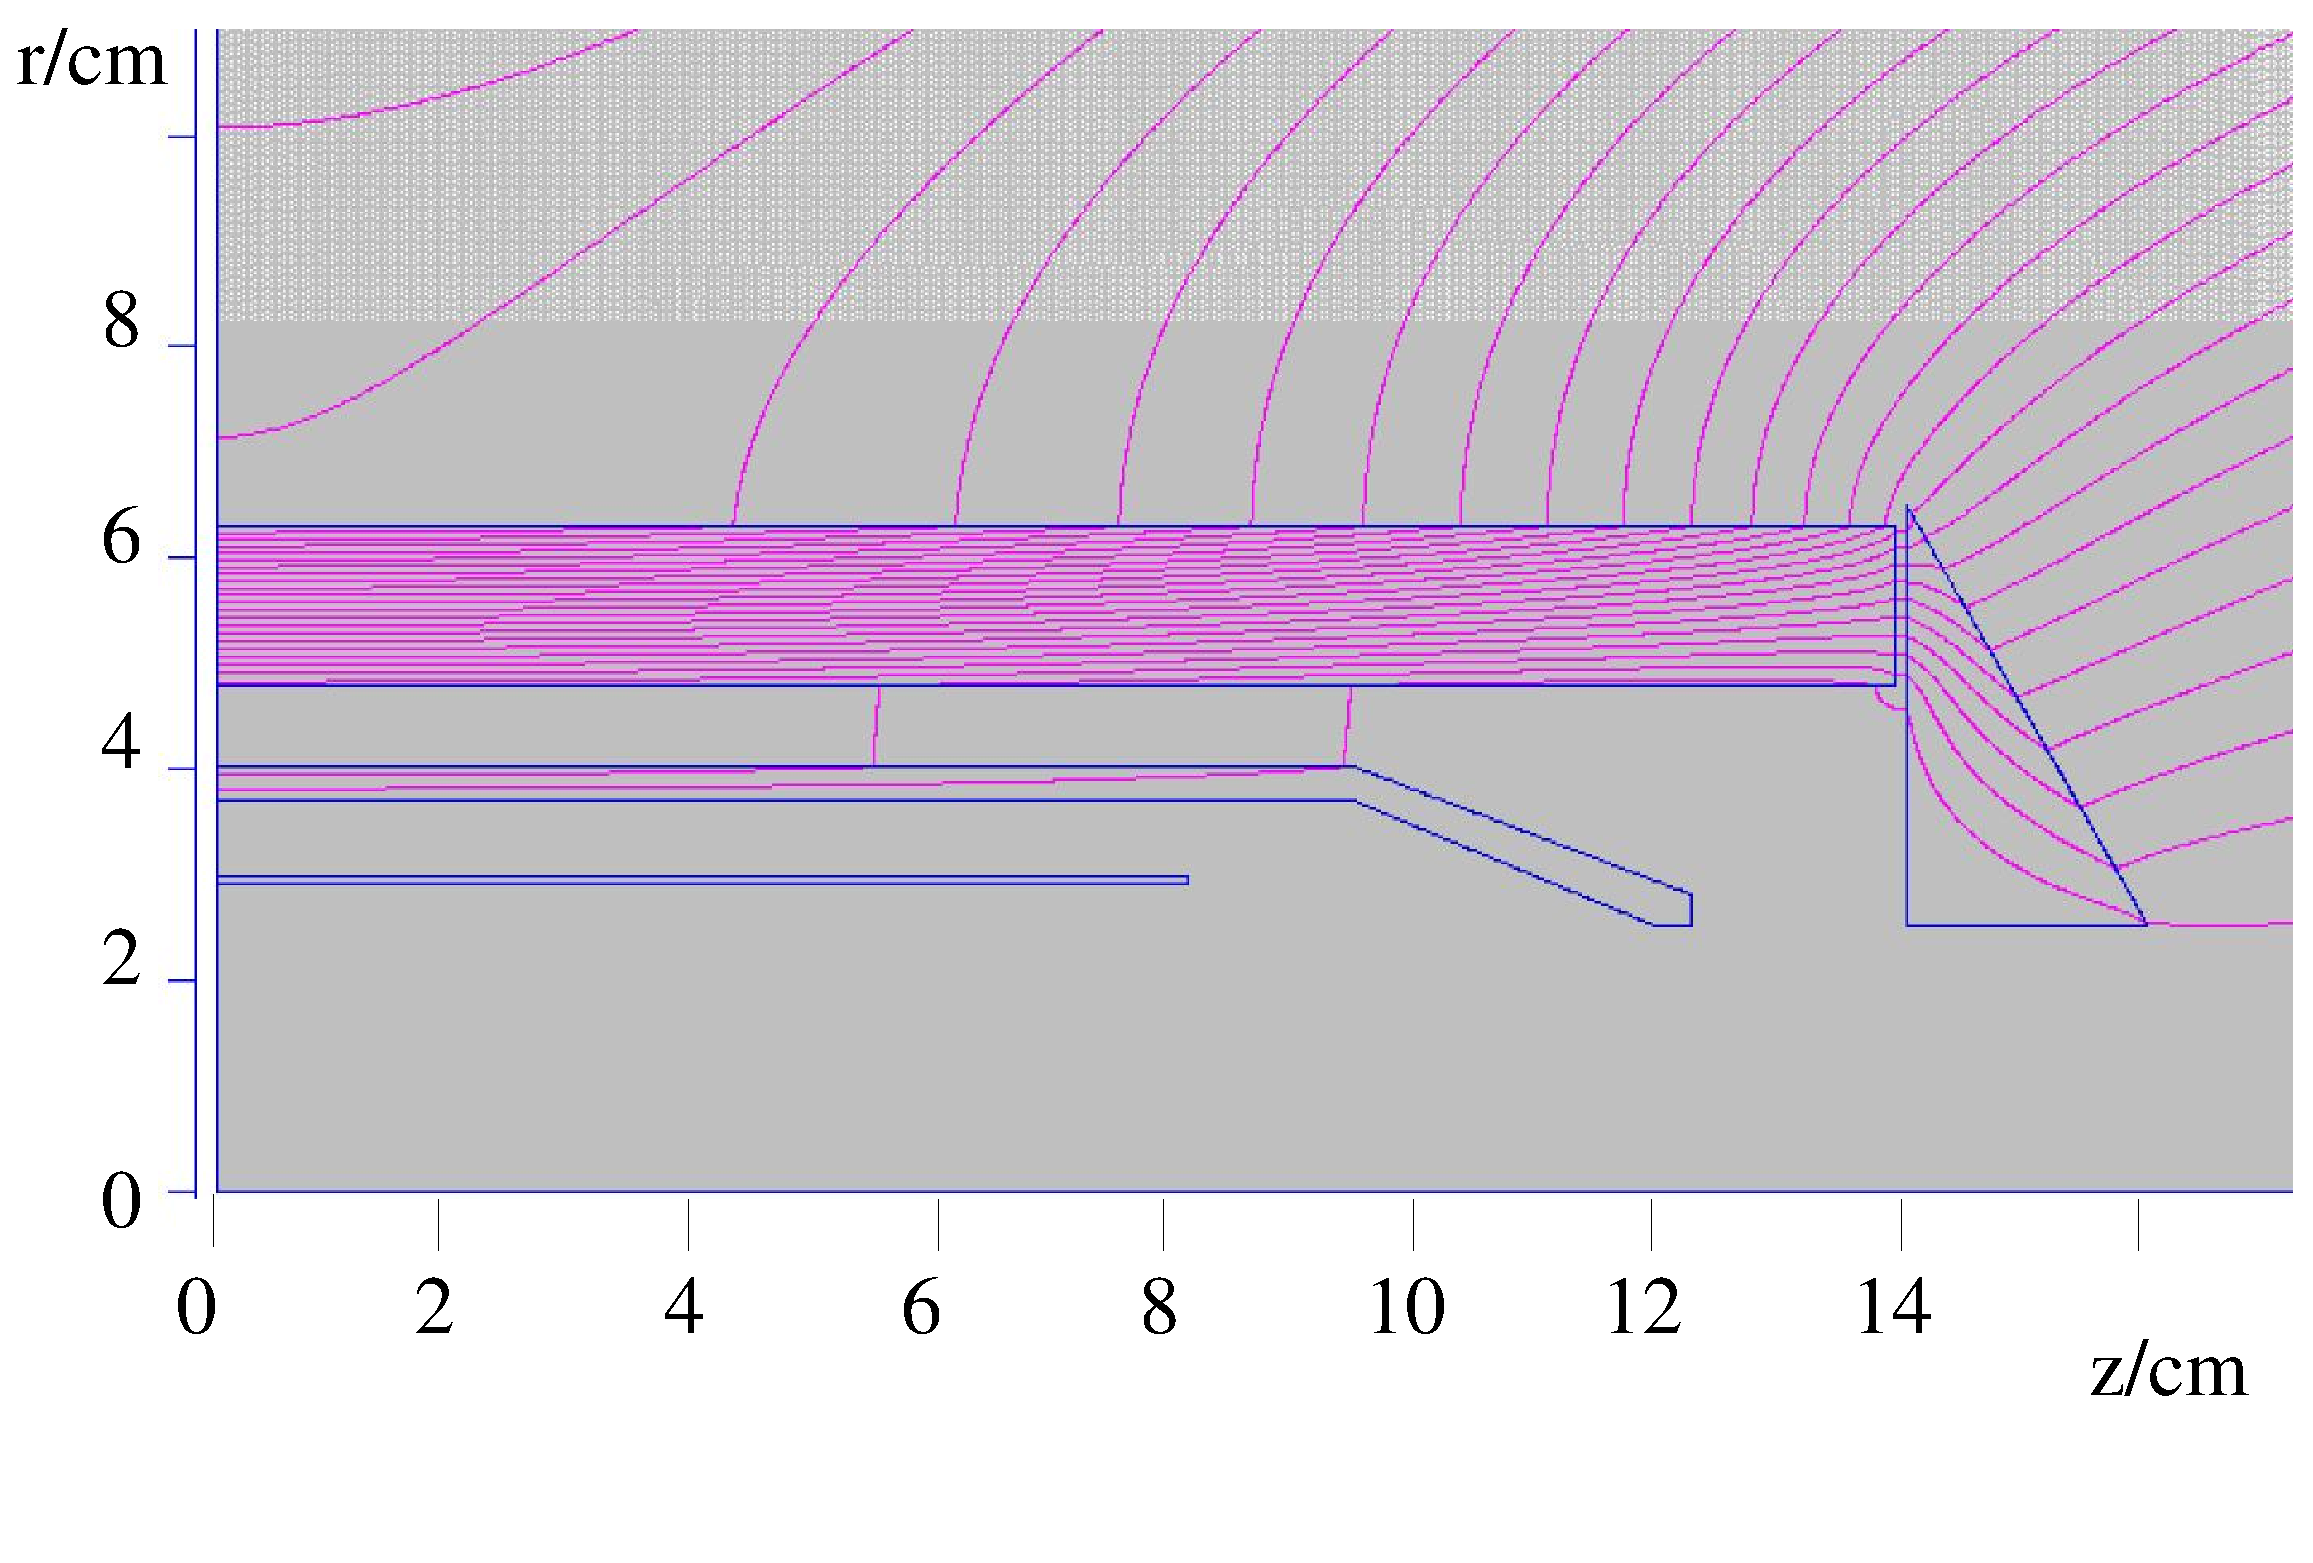
\includegraphics[height=5cm]{R2083_NETIC_hiperm49_CONETIC_standardDesign.eps}
\label{R2083_Initial}}
\qquad
\subfloat[]
	{\includegraphics[height=5cm]{R2083_Iron_hiperm49_CONETIC_0.3mm_PMT_Region.eps}
\label{R2083_Initial_NETIC_PMT_Region}}
\qquad
\caption{\small{(a) Triple layer ferromagnetic shielding at 1000~G.
(b)-Magnetic fields in the {\tt PMT} region.}}\label{R2083_Initial_Iron}
\end{figure}

A quarter of {\tt PMT}  occupies a box with $(z,r)$
-coordinate $(0,0)$ and $(4.5,2.3)~cm$,  
while the  photo cathode is located at  $z=4.5~cm$. 
We remind that   fringe  fields  of  $0.2~G$ were 
admitted to be critical  for  timing {\tt PMT}s. 
According to this map, unfortunately,  the central  
field is  about $0.5~G$. 
Moreover,  it  increase towards   open ends of the shield, due to a
penetrating  axial field lines. At the photo cathode it is
higher of $0.8~G$.  


However, on hope to find a better combination, shields 
with different  external materials were further 
tested at varying magnetic fields, from $250~G$ to $1250~G$.
Doing so we  monitor the following  
points\footnote{All points are given in $(r,z)$ form and are 
expressed in $cm$.} 
inside the sensitive region of a {\tt PMT}:$(0,0)$ and $(2.3,0)$ 
at  the median plane where the  first {\tt PMT} dynode is situated;
$(0,5)$ and $(2.3,5)$ at  the {\tt PMT} photo cathode.
In order to control  saturation effects we monitor 
the bulk of ferro-magnetics as well.
%\paragraph{Calculations and results.}
The result of such tests is shown in 
Fig.~\ref{R2083_Initial_Iron_PMT_Region}.

In all four points of interest  the inner field  rise  up, 
slowly, up to external field of  $750~G$, 
then, at higher external fields, 
it climbs rapidly. The behavior of
bulk ferromagnetic fields indicates this effect 
as due to a  saturation of the external  layer. 

The  external  field  $750~G$ has been  depressed up 
to $0.4-0.9~G$ within the {\tt PMT} volume. 
Using  {\tt NETIC} for the  external layer results in $\approx20\%$ 
higher critical field, only.  
The  residual fields  still remain within the same interval.
In hope to reduce the inner fields, we have increased 
the thickness of the middle layer up to $8~mm$, 
that additionally  improved the critical field by another $20-30\%$,
but did not improve the shielding performance.

All these tests show 
quite low inner field. However, in all cases it  remains  
significantly  higher of the  tolerable limit,   even 
at  lowest external field of $250~G$.  
Moreover, the outer shield layer is already  reached  its maximum 
thickness as allowed by the current {\tt CTOF} design.
  

Hence, we conclude that  the  Triple Ferromagnetic Shielding  is  not  
sufficient  in the environments of the {\tt CTOF} detector.
It looks like  the last resort of ferromagnetic shields is  
exhausted  under the 
burden of design constrains.
However, we have succeeded to  find a solution.
 
In the following Section~\ref{sec:novelle} we describe a novel 
ferromagnetic shield which 
allows  to attain fields below $0.1~G$ in both  upstream and
downstream {\tt PMT}s at  axial fields of $1000~G$.

\section{Novel Dynamical Magnetic Shields.}
\label{sec:novelle}

As it was shown in Section~\ref{sec:ednmics} the inner 
field of a shielding cylinder
is determined by the   magnetization  of a ferromagnetic material.  
Our main idea is to control the magnetization of the innermost 
shield cylinder, using active elements, such as solenoid. 
The  solenoid  is  wind  around a ferromagnetic component, 
i.e. it is placed outside the 
shielding cylinder.  Its  current
is set to reduce the  magnetization of the ferromagnetic. 
Thus, the field inside the cylinder is also 
reduced following to boundary conditions at the  
inner surface of the ferromagnetic.

We call this  combination  of passive  and active shielding 
elements  as ``hybrid~shield'' or 
``dynamical~shield''. In the following Section~\ref{sec:tests}  
we show that with such shields  
it is possible to  attaining inner fields below $0.2~G$
at axial fields high as $1000~G$.

We notice that would one  place the solenoid  $inside$ the cylinder, 
the  effect could  be even opposite to expectations.
Point is that in such a case%5
 
the additional   magnetization of the  external  
ferromagnetic is opposite to the compensating field. 
Therefore, $decreasing~inner~field$  is accompanied with 
$increasing~magnetization$ of the external ferromagnetic.
The last   even  may  saturate at certain  
current of demagnetizing solenoid.

 
Hence, numerous {\tt POISSON} calculations have convinced us that
two opposite  fields
%, i.e.the  inner solenoid field and  the inner  field 
%of external cylinder, 
do not compromise in the {\tt PMT} area.
Typically  the  result is  a significantly $higher$ inner field with frequent
``collapse`` owing to a saturated layer. 

On Fig.~\ref{VBT3CYUS1} we present the viable  design and the corresponding field map  
for the Hybrid Magnetic Shield with a demagnetizing  solenoid inside the assembly. 
The coil with ~100 winds of ~$1 mm$-wire  is placed between the  middle and  the 
inner layers. The current through the coil wire is  below 1~A  that allows to avoid overheating.  
A more detailed  field map inside the PMT region at 400~G  is 
shown in Fig.~\ref{VBT3CYUS2}. According to this figure, the demagnetizing  coil 
allows   optimized   inner {\tt PMT} field  to be  below  0.1~G.
Moreover, the field  magnitude is quite uniform within a wide area.

\begin{figure}[ht]%001
\centering
\subfloat[]
	{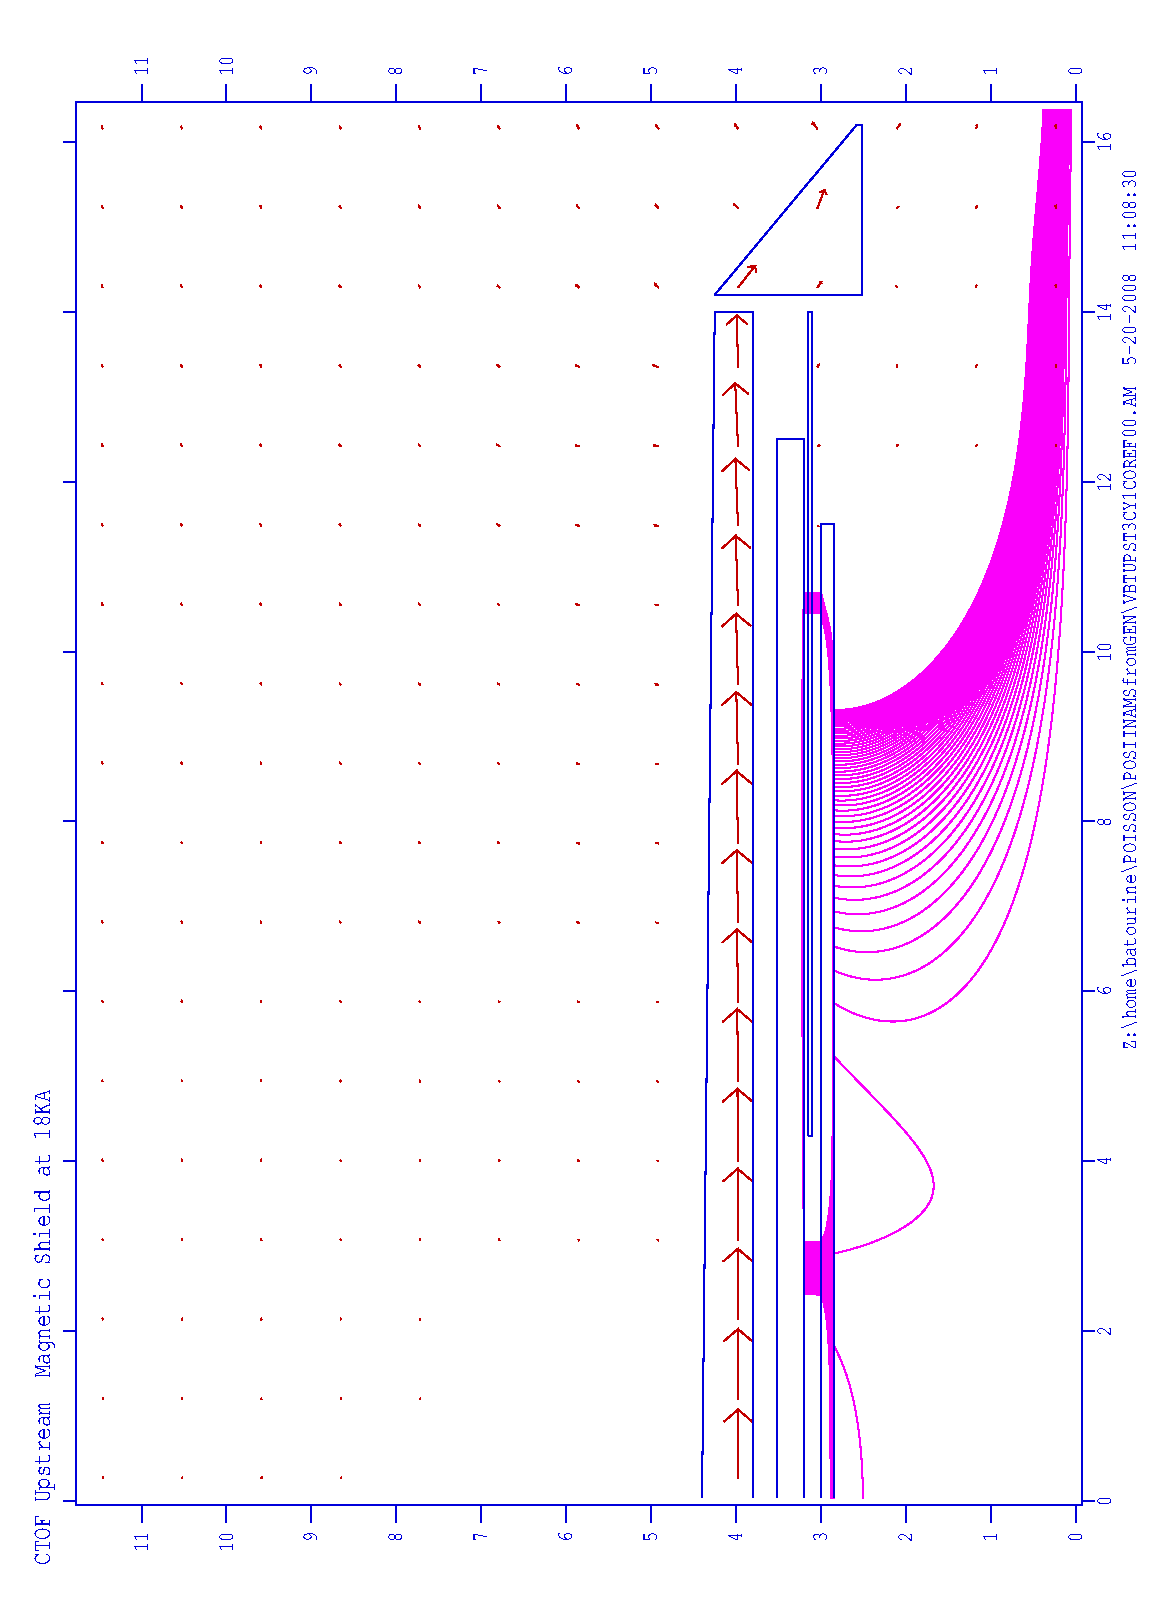
\includegraphics[height=7cm]{VBTUPST3CY1COREF0001.eps}\label{VBT3CYUS1}}
\qquad
\subfloat[]
        {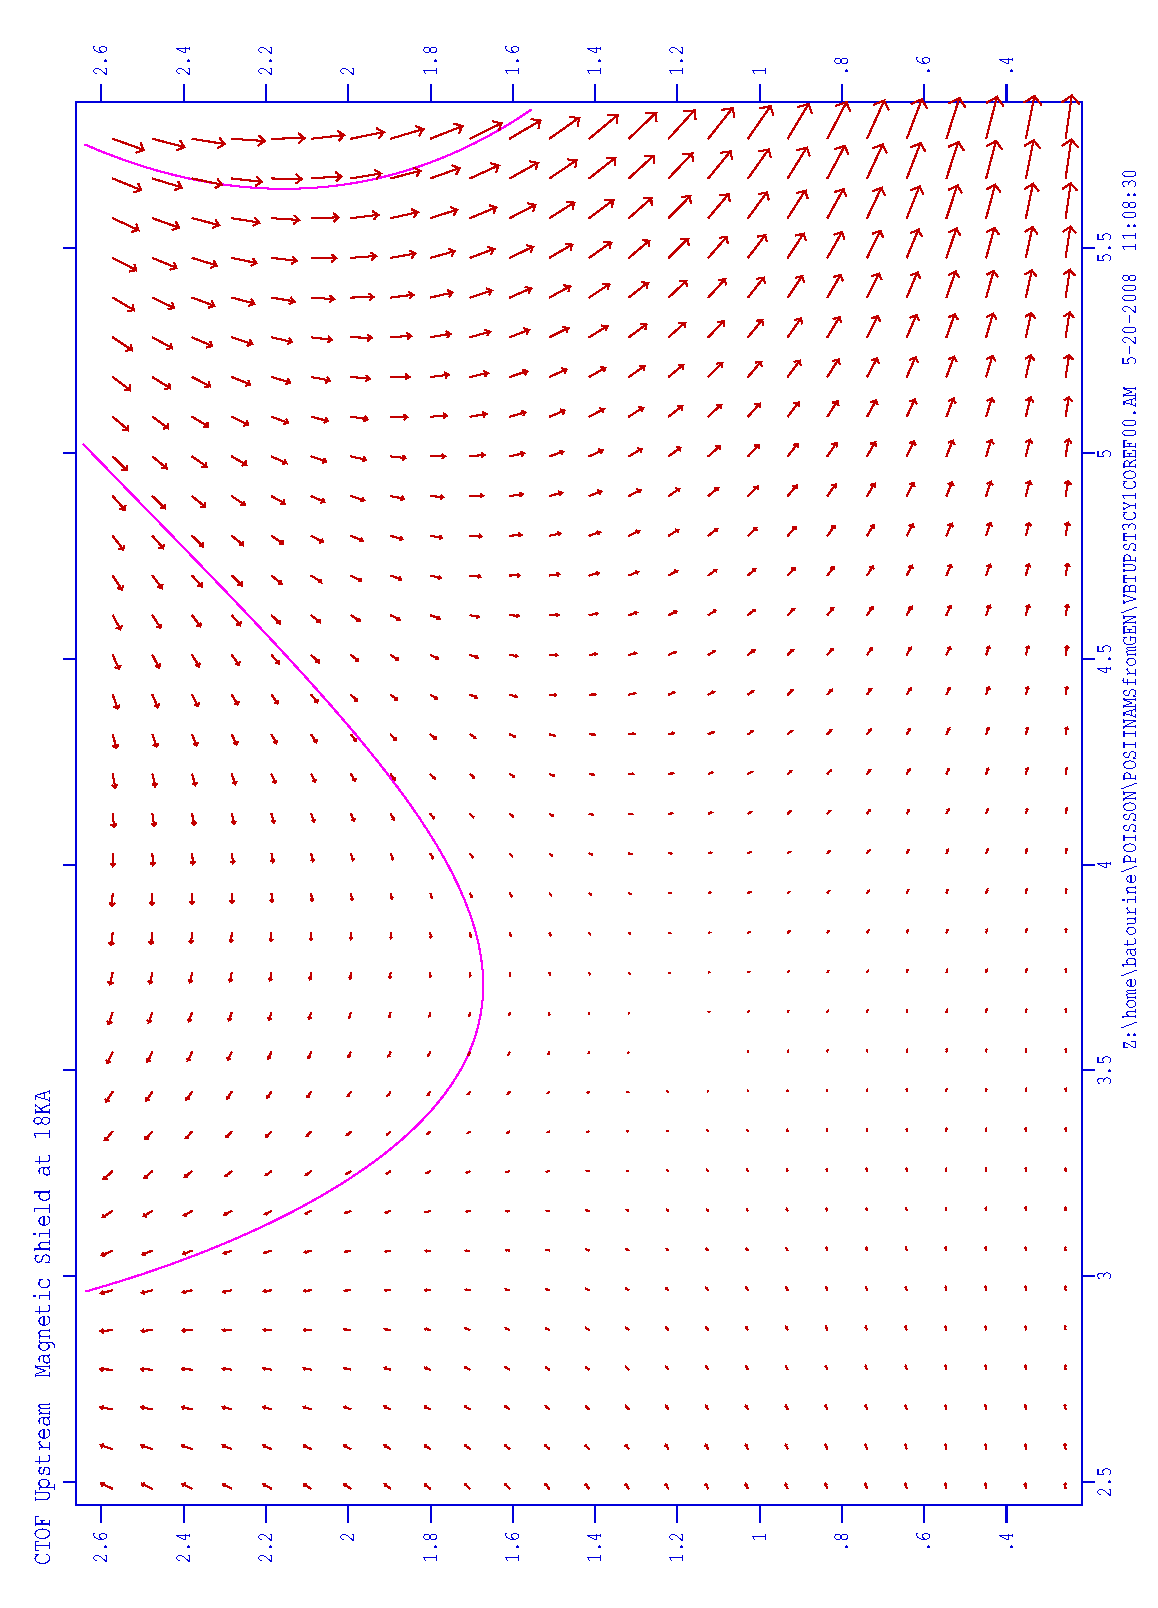
\includegraphics[height=7cm]{VBTUPST3CY1COREF0002.eps}\label{VBT3CYUS2}}
\caption{\small{(a) Hybrid Magnetic Shield in  $400~G$-field. 
Vertical scale -$z/cm$; horizontal scale-$r/cm$.
(b) Zoomed-in field map in the {\tt PMT} area.
Arrow lengths indicate  field magnitudes; 
the longest  arrow  is for  $1~G$.}}
\end{figure}

%\subsection{Upstream dynamical shield.}
The  shield shown in Fig.~\ref{VBT3CYUS1}  may be used at the 
upstream side of the {\tt CTOF} detector at  400~G provided 
the light guides are about $1.5~m$ long. 
It is obvious from  {\tt POISSON} calculation that  higher fields may be  
exterminated with a thicker outer layer and/or 
higher currents in the  coil, 
provided that external ferromagnetic does not saturates.
Thus, Dynamical  Magnetic Shield looks  very promising. 
Therefore we have  further  developed   and  prototyped  such shield.
Below we describe our first real Dynamical Shield  and 
experimental tests using this shield.

\subsection{Tapered Dynamical Shield.}
\label{sec:tapered}
In our previous calculations, it was observed that the 
bulk  field  in the outermost shielding layer was 
non-uniform across the length of the shield, becoming greater
towards the median of the cylinder.
This effect may be seen from any calculated field map as follows.
For example, in Fig.~\ref{R2083_Initial}
we observe that field lines are captured  by the outer cylinder almost 
normal to its surface. Then, due to a very high permeability, all filed lines
run  almost parallel to the axis. Therefore  magnetic flux density 
increase, roughly linearly, towards the median of the cylinder. 
Thus, the  most critical  place, where the  effect of  ferromagnetic saturation 
shows up first, is just  the median plane.  In the vicinity of the  median plane 
the external field lines are almost perpendicular. 
Therefore they efficiently penetrate through a ``gap'' created by a 
saturated ferromagnetic into the {\tt PMT} area, that explains the 
shield performance collapse with  increasing  shield length. 

In order to make magnetization more uniform across the ferromagnetic 
and avoid such saturation effects
we suggest an improved  design. This design  involves the use 
of a tapered outer cylinder,
the  thickness of which  linearly increase  towards the median plane.

%\paragraph{Design.}
The design with tapered outer cylinder, in combination with the demagnetizing 
coil  between two innermost layers, is shown in  Fig.~\ref{Tapered_Shield_Design}.
The outermost  shield is composed of Soft Iron, 
beginning with a thickness of $1.0~cm$ and 
slowly thickening to $1.7~cm$. 
The middle layer is made of Hiperm49 $3~mm$ thick while  
the inner layer is {\tt CO-NETIC} $0.8~mm$ thick.
%\paragraph{Performance.}

The performance of this  shield 
was studied first  with {\tt POISSON}  at  external solenoidal  field 1000~G and 
varying current through the compensating coil. 
As in our previous tests, we  monitor field values inside {\tt PMT} in several reference points.

The resulting fields in function upon the coil current 
are shown in  Fig.~\ref{Tapered_Shield_0.3cm_PMT_Region}.
It is observed that the internal magnetic field of the {\tt PMT} 
region is of $0.1~G$ 
at the  coil 
current\footnote{ {\tt POISON} model specifies the total  
current through the $(r,z)$-plane in $A$$\times$$Winds$.}
of $20-30$~AW.
It is also of interest to note that at this high magnetic field,
none of three ferromagnetic cylinders have reached saturation.
Additionally, the magnetic flux density within the {\tt PMT} region is much more uniform
than previously observed.

Thus, the dynamical shield   is an  excellent candidate 
to the {\tt PMT} shield in  the {\tt CTOF} detector.
%
\begin{figure}[htbp]%[ht]%
\centering
\subfloat[]
{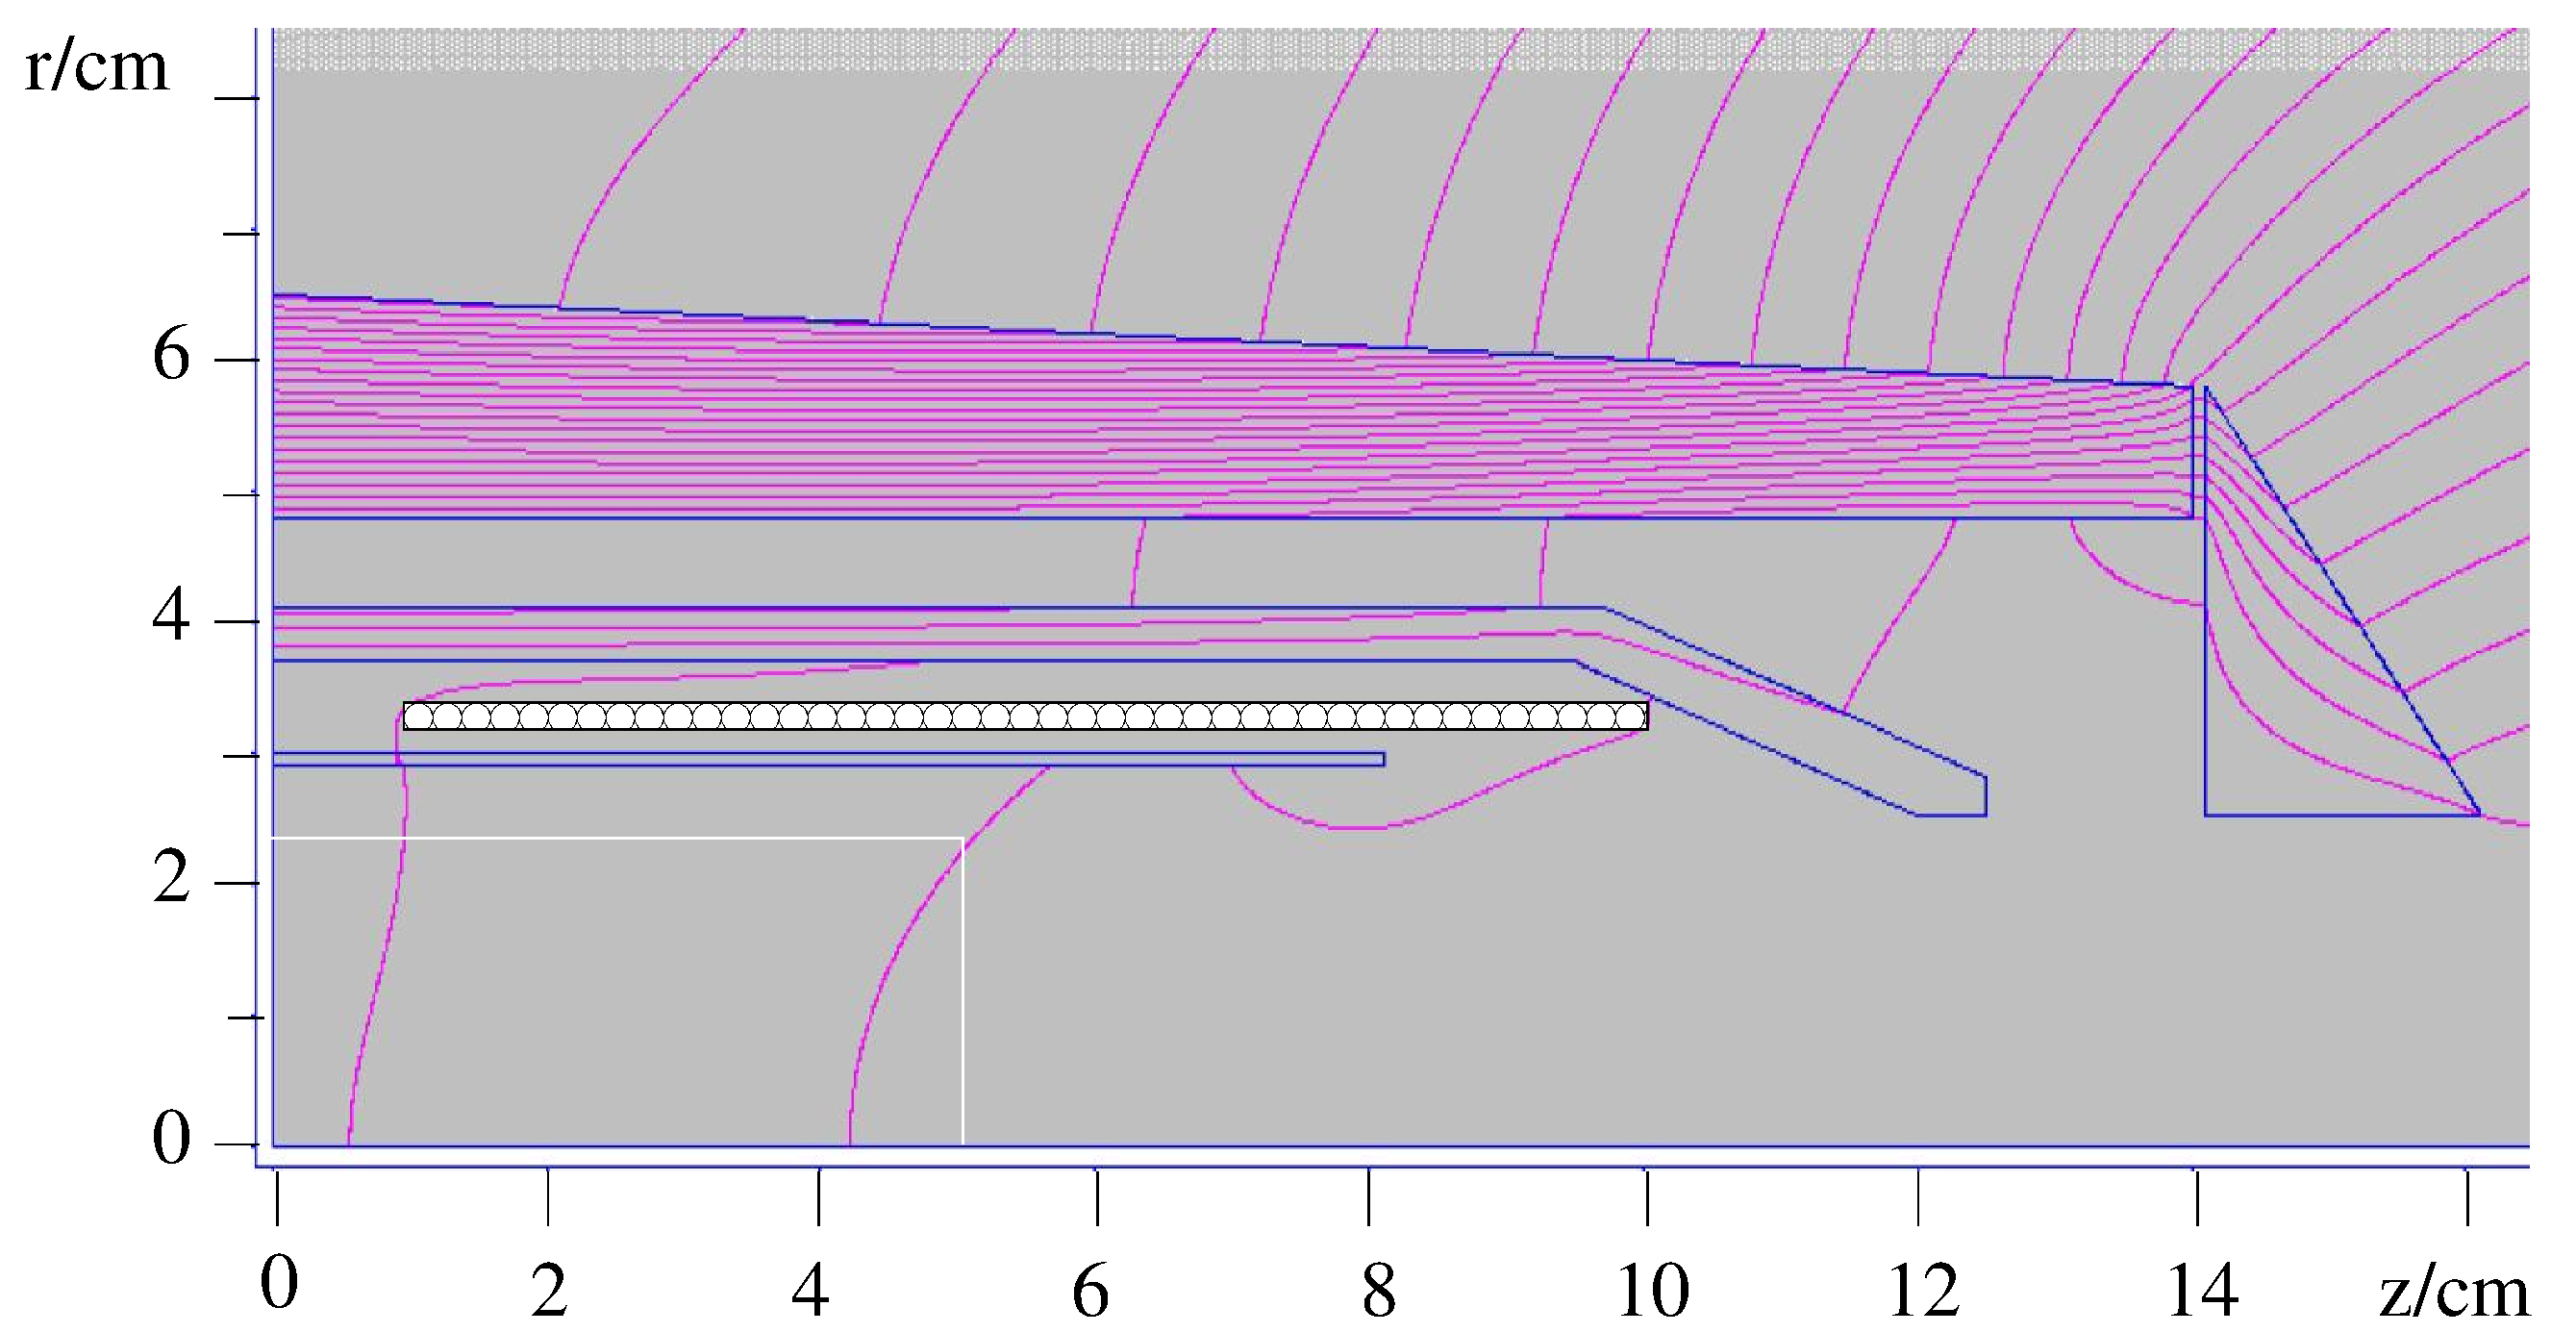
\includegraphics[height=4cm]{R2083_Iron_hiperm49_CONETIC_TaperedShieldDesign.eps}\label{Tapered_Shield_Design}}
\qquad
\subfloat[]	
{\includegraphics[height=5cm]{R2083_Tapered_0.3cmMiddle_PMT_Region.eps}\label{Tapered_Shield_0.3cm_PMT_Region}}
\caption{\small{
(a)~Tapered Dynamical Magnetic Shield. The outermost tapered cylinder is ~Iron  10-17~mm thick.
 Middle cylinder is ~Hiperm-49 3~mm thick. Inner cylinder is ~{\tt CO-NETIC} 0.8~mm thick.  
The external Solenoid runs  at 1000~G. Correction coil current is set to 25~A.
(b)~Magnetic field in the  {\tt PMT} region.}  in function on the coil current.}
\label{Tapered_Shield_0.3cm}
\end{figure}
%\newpage




\subsection{Prototyping and Testing.}
\label{sec:tests}
In this section  we describe the  realistic   prototype of the Dynamical Magnetic Shield.
Its  design corresponds to the one Fig.\ref{Tapered_Shield_0.3cm} and
 described in the previous Section\ref{sec:tapered}.
The outermost shield layer was fabricated from very common 1018 steel. The innermost 
ferromagnetic was made of mu-metal, which is slightly worse ferromagnetic than  {\tt CO-NETIC}.
The middle layer material is Hyperm49. 
The prototype was placed inside the center of the 130~mm-bore 
of  the Super Conducting Solenoid.
 The solenoidal  field within the space occupied by the prototype was almost
 uniform by the  magnitude.

%The almost uniform external field was produced by the Helmholtz coils 2~m in diameter. 
Axial and radial Hall-probes of Gauss-meter were stepped  along and across 
the PMT space  with  1~cm-increment. The performance of DMS was tested  up to the  ultimate  
field 908~G. 
Thus measured  inner field profiles at ultimate field are shown in Fig.\ref{innergauss}.
%Thus, our practical tests show the vitality of
%the idea of using compensating coils. 
%The practical realisation of such 
%shielding is quite  easy. 
%The shield  shown in Fig.~\ref{VBT3CYUS1} has a compensating coil wind around the innermost cylinders.
%This shield has demonstrated  a good performance in  simulations  and experimental tests.
%Therefore, it is  considered  as a prototype for the    the Upstream {\tt R2083} shield.
%
\begin{figure}[ht]%002
\centering
\subfloat[]
	{\includegraphics[height=5cm]{shield908axialprobe.eps}\label{axiprob}}
\qquad
\subfloat[]
{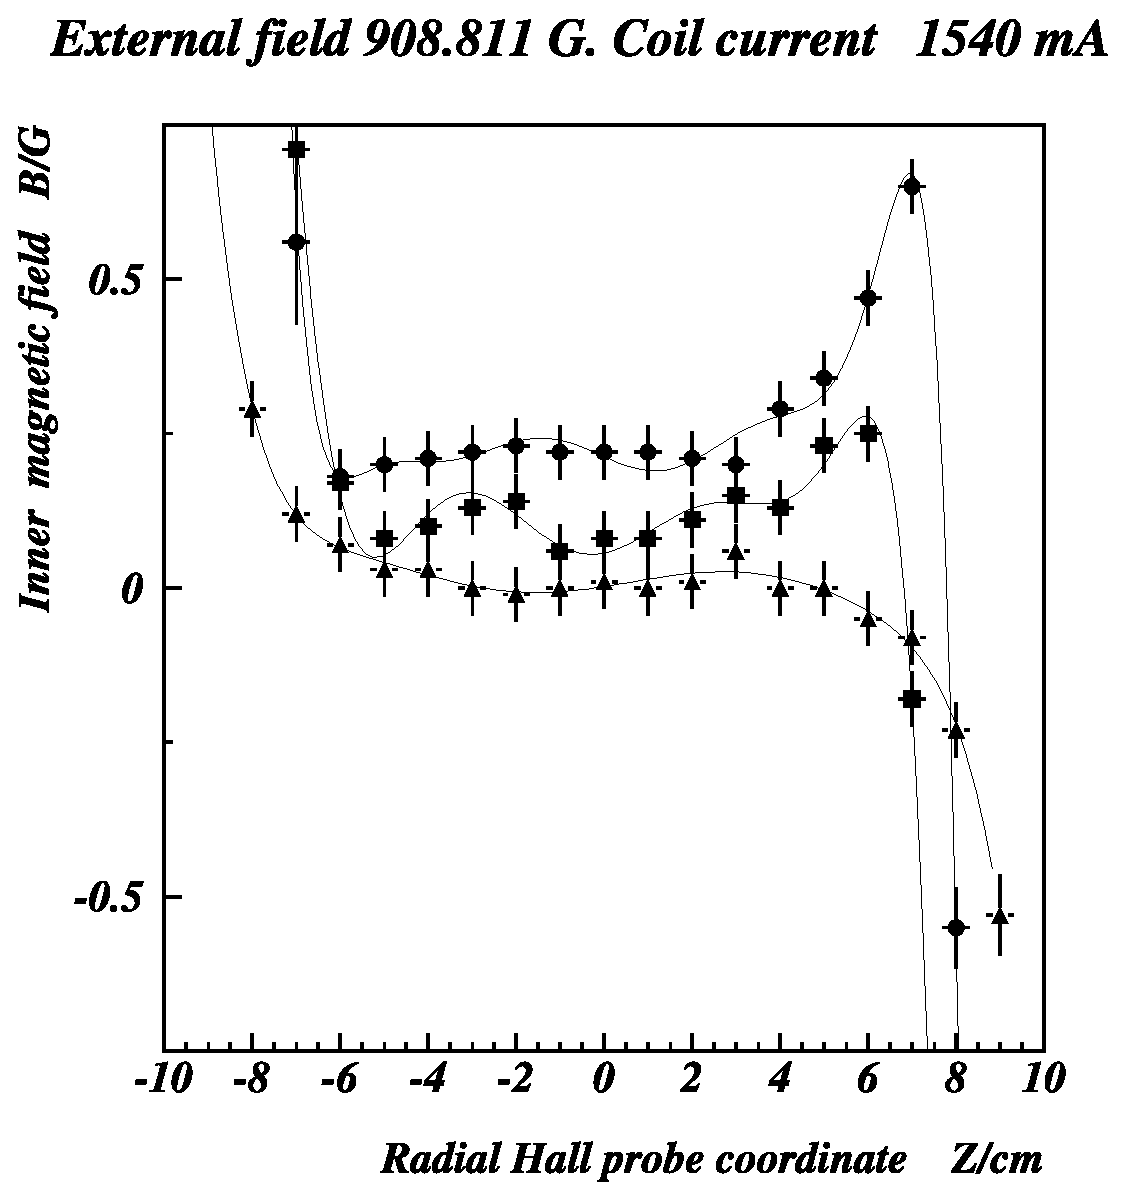
\includegraphics[height=5cm]{shield908radialprobe.eps}\label{radprob}}
\caption{\small{Measured inner field of the Dynamical  Magnetic Shield
in  the external  solenoidal field 908~G.
 Axial~(a) and radial~(b) component of the inner field at coil current 15.4~AW.}
\label{innergauss}}
\end{figure}

In this figure  the novel Dynamical Magnetic Shield demonstrates 
 a good performance in experimental tests. At demagnetizing current of 15~AW
both components, radial shown in Fig.\ref{axiprob} and axial in Fig.\ref{radprob}, 
are within the tolerable  interval (0,0.2)~Gauss.
Considering that permeability of ferromagnetic samples may differ from their model specifications, 
 these results, i.e. field magnitudes and demagnetizing current, 
 may be qualified to be in good accordance to the {\tt FEA}  from Section~\ref{sec:tapered}.

The corresponding to the tolerable interval   area is a  cylinder sized as 
$4\times10 cm^2$. It  is sufficient to house the accelerating system of 
our reference  photo multiplier  {\tt R2083} from Hamamatsu.
Further increase of external  field beyond $920~G$ results in rapid climbing  of inner fields 
due to  ferromagnetic saturation.
Using better steel, such as 1008 or 1006 will definitely result in higher tolerated fields.

\section{Conclusion.}
\label{sec:concl}
We have developed a simple theory of ferromagnetic  shield in axial fields.
Numerous {\tt FEA} calculations were also  performed for various shields for both upstream and 
downstream regions of the {\tt CTOF} detector. 
These calculations have demonstrated that the dynamics of coaxial   
ferromagnetic cylinders is very
complex. Some  unexpected effects were manifested by the models, 
such as  performance  
collapse with increasing  length.  
This effect was predicted  by our simple   theory.
Hence, this  simple theory allows a  clear and unambiguous   interpretation of  
{\tt FEA} calculations, sometimes surprising, in relation to the  designing of real shields.

With the  help of the {\tt POISSON} program we have designed a  single layer  ferromagnetic 
shield which  may sufficiently protects  metal channel {\tt PMT}s  up to high axial 
fields of $2500~G$.   
                                                        
Given the restrictions from the  design with {\tt R2083} {\tt PMT}s 
the best possible configuration for the triple ferromagnetic  shield was found. 
However, even such advanced  shield
will  be effective  to satisfy the stringent $0.4~G$ tolerance, only.
In order to  attain fields below $0.1~G$ we have developed a novel 
Dynamical Magnetic Shield which consists  of ferro-magnetics layers 
and solenoids  between the layers. 
Such shield was tested within  {\tt POISSON} models  
and experimentally.  The Dynamical Shield  has demonstrated  excellent  performance.   
Additional advantage of more uniform field inside a {\tt PMT} 
has been achieved by a tapered design of the external cylinder. 

\paragraph{Acknowledgments.}We appreciate Dr. E.~Chudakov for helping in   
{\tt POISSON} model setup  and valuable advices. 
We also express our gratitude to Dr. C.Keight and his 
team for the  technical  support of  shield testing.


\section{Bibliography}
%\input{references.tex}
\begin{thebibliography}{99}

\bibitem{upgrade2} 
{\tt CLAS12} Technical Design Report 2009.

\bibitem{flint} 
J.Flint and E.Smith,% ``Tests of Phillips XP4312/D1 PMTs in a Magnetic 
Field'', CLAS-Note-94-008,(1994)

\bibitem{r2} 
E.S.Smith {\it et al.},% ``The Time-of-Flight System for CLAS'',  
Nucl. Instr. and Meth. A {\bf 432}, 265 (1999).

\bibitem{r1} 
V.N.Batourine {\it et al.}, %``Measurements of PMT Time Resolution at Kyungpook National University'', 
CLAS-NOTE~2004-16, (2004),

\bibitem{cn200439} 
V.N.Batourine {\it et al.}. %``Studies of Time Resolution of the Burle 85001 Micro-channel Plate Photomultipliers in Comparison with Standard PMTs'',
CLAS-NOTE~2004-39, (2004).

\bibitem{llg}  
V.Batourine {\it et al.}.% ``Status Report on the Studies at Kyungpook National University in 2005'',
CLAS-NOTE~2005-3, (2005).

\bibitem{cn85011}  
F.Barbosa {\it et al.},% ``Status and Further Steps Towards the CLAS12 
%Start Counter'', 
CLAS-NOTE~2006-011, (2006).

\bibitem{Baturin:2005} 
V.Baturin {\it et al.},% ``Time-of-Flight Resolution of Scintillating Counters with Burle 85001 Micro-channel Plate Photomultipliers in Comparison with Hamamatsu R2083'', 
Nucl. Instr. and Meth. A {\bf 562},327(2006).

\bibitem{6percent} 
V.Baturin {\it et al.},% ``Time Resolution Measurements with the Final Prototype for the CLAS12 Central TOF Detector.'', 
CLAS-NOTE~2009-001,(2009).

%\bibitem{elton Gluex-doc-843 Jul-17 by E.Smith}

\bibitem{dynshi} 
V.Baturin {\it et al.},% ``Dynamic Magnetic Shields for the CLAS12 Central TOF Detector'', 
CLAS-NOTE~2008-034,(2009).

\bibitem{wieland}
B.M.Wieland,% ``Advanced Studies of the Photomultiplier Tube Magnetic Shielding for the CLAS12 Central Time of Flight Counter", Old Dominion University, 
Senior Thesis,Old Dominion University,2009.

\end{thebibliography}

\end{document}


